\documentclass[12pt,a4paper]{article}

% Paquetes de configuración del documento
\usepackage[utf8]{inputenc}
\usepackage[spanish]{babel}
\usepackage[T1]{fontenc}
\usepackage{siunitx}
\usepackage[margin=2.5cm]{geometry}
\usepackage{fancyhdr}
%Paquetes para simbologia%
\usepackage{amsmath}
\usepackage{amsfonts}
\usepackage{amssymb}
\usepackage{physics}
\usepackage{longtable}
\usepackage{graphicx}
\usepackage{caption}
\usepackage{float}
\usepackage{xurl}
\usepackage[colorlinks=true,
            linkcolor=black,
            urlcolor=myblue,
            citecolor=black,
            filecolor=black]{hyperref}
 % Opción estándar para enlaces
\Urlmuskip=0mu plus 1mu          % Mejora el espaciado para permitir cortes
\usepackage{subcaption}  % en el preámbulo
\usepackage{pgfplots}
\usepackage{pdfpages}
\pgfplotsset{compat=1.18}
\usepackage{tikz}
\usepackage{xcolor}
\definecolor{myblue}{RGB}{42, 127, 179}


% Encabezado
\pagestyle{fancy}
\lhead{\textit{Ingeniería Mecánica}}
\chead{\textit{Materiales Metálicos}}
\rhead{\textit{UTN-FRVM}}

\begin{document}
\begin{titlepage}
	
	\begin{center}
		{\huge \textit{Universidad Tecnológica Nacional}}\\
        \vspace{0.5cm}
		{\LARGE \textit{Facultad Regional Villa María}}\\
		\vspace{1.5cm}
        {\LARGE{\textit{Ingeniería Mecánica - Materiales Metálicos}}}\\
		\vspace{1.5cm}
        \LARGE{\textit{Trabajo Práctico 3-06}}
	\end{center}
	
	\vfill

    \textit{Grupo DEL RÍO:}
	\begin{itemize}
		\item \textit{Abregú, Iván.}
		\item \textit{Antico, Rodrigo.}
		\item \textit{Brussa,Julián.}
		\item \textit{Cabral, Franco.}
        \item \textit{Cárdenas, Felipe.}
        \item \textit{Cardozo, Martín.}
        \item \textit{Córdoba, Nathan.}
        \item \textit{Cucco, Ramiro.}
        \item \textit{del Río, Juan.}
        \item \textit{Guerini, Nazareno.}
        \item \textit{Medina, Ivo.}
        \item \textit{Ortiz, Gastón.}
        \item \textit{Picos, Elías.}
        \item \textit{Quinteros, Lautaro.}
	\end{itemize}
    
	\textit{Docentes:}
	\begin{itemize}
		\item \textit{Dr. Lucioni, Eldo José.}
		\item \textit{Ing. Victorio Vallaro, Juan Manuel.}
	\end{itemize}
	\centering
	\today
	
\end{titlepage}

\tableofcontents

\begin{abstract}
    \underline{\textbf{Requerimiento del Trabajo:}} Investigue los métodos de obtención de arrabio, acero y fundición a fin de adquirir la capacidad de explicar conceptualmente los mismos. La actividad requerida incluye la identificación del tipo y uso de los hornos asociados a dichos métodos de obtención. [NOTA: A modo de orientación, puede consultar la siguiente fuente de información:]
    \begin{itemize}
        \item Aguilar Schafer, J.A. Yacimientos minerales y procesos geológicos.
        \item Aguilar Schafer, J.A. Explotación minera, preparación y concentración.
        \item Aguilar Schafer, J.A. Metalurgia extractiva del hierro.
        \item Aguilar Schafer, J.A. Hornos Industriales.
    \end{itemize}
\end{abstract}

\section{Introducción.}
Antes de comenzar a explicar cómo se obtiene el arrabio, el acero, la fundición y qué hornos están asociados con la obtención de cada uno, primero vamos a definir una serie de términos que son importantes para entender de que estamos hablando. También cabe destacar que sólo nos concentraremos en la obtención de los tres materiales mencionados, sus materias primas y la descripción de los hornos correspondientes a la fabricación, dejando de lado cuestiones que tienen que ver con la minería y la obtención de la materia prima.

\subsection{Arrabio.}
\begin{itemize}
    \item \textbf{¿Qué es?}
\end{itemize}

El arrabio es el producto metálico intermedio que se obtiene de la reducción de los minerales de hierro en el alto horno (En la sección \hyperref[alto_horno]{2.2} se explicará más a detalle). Es una aleación de hierro con un alto contenido de carbono, normalmente entre 3\% y 4,5\%, y que además incluye impurezas como silicio, fósforo, manganeso y azufre. El nombre “arrabio” proviene del antiguo término “hierro bruto”, ya que se trata de un material inicial que no tiene aplicación directa salvo como materia prima para fabricar acero o fundición.

\begin{figure}[H]    
    \centering         
    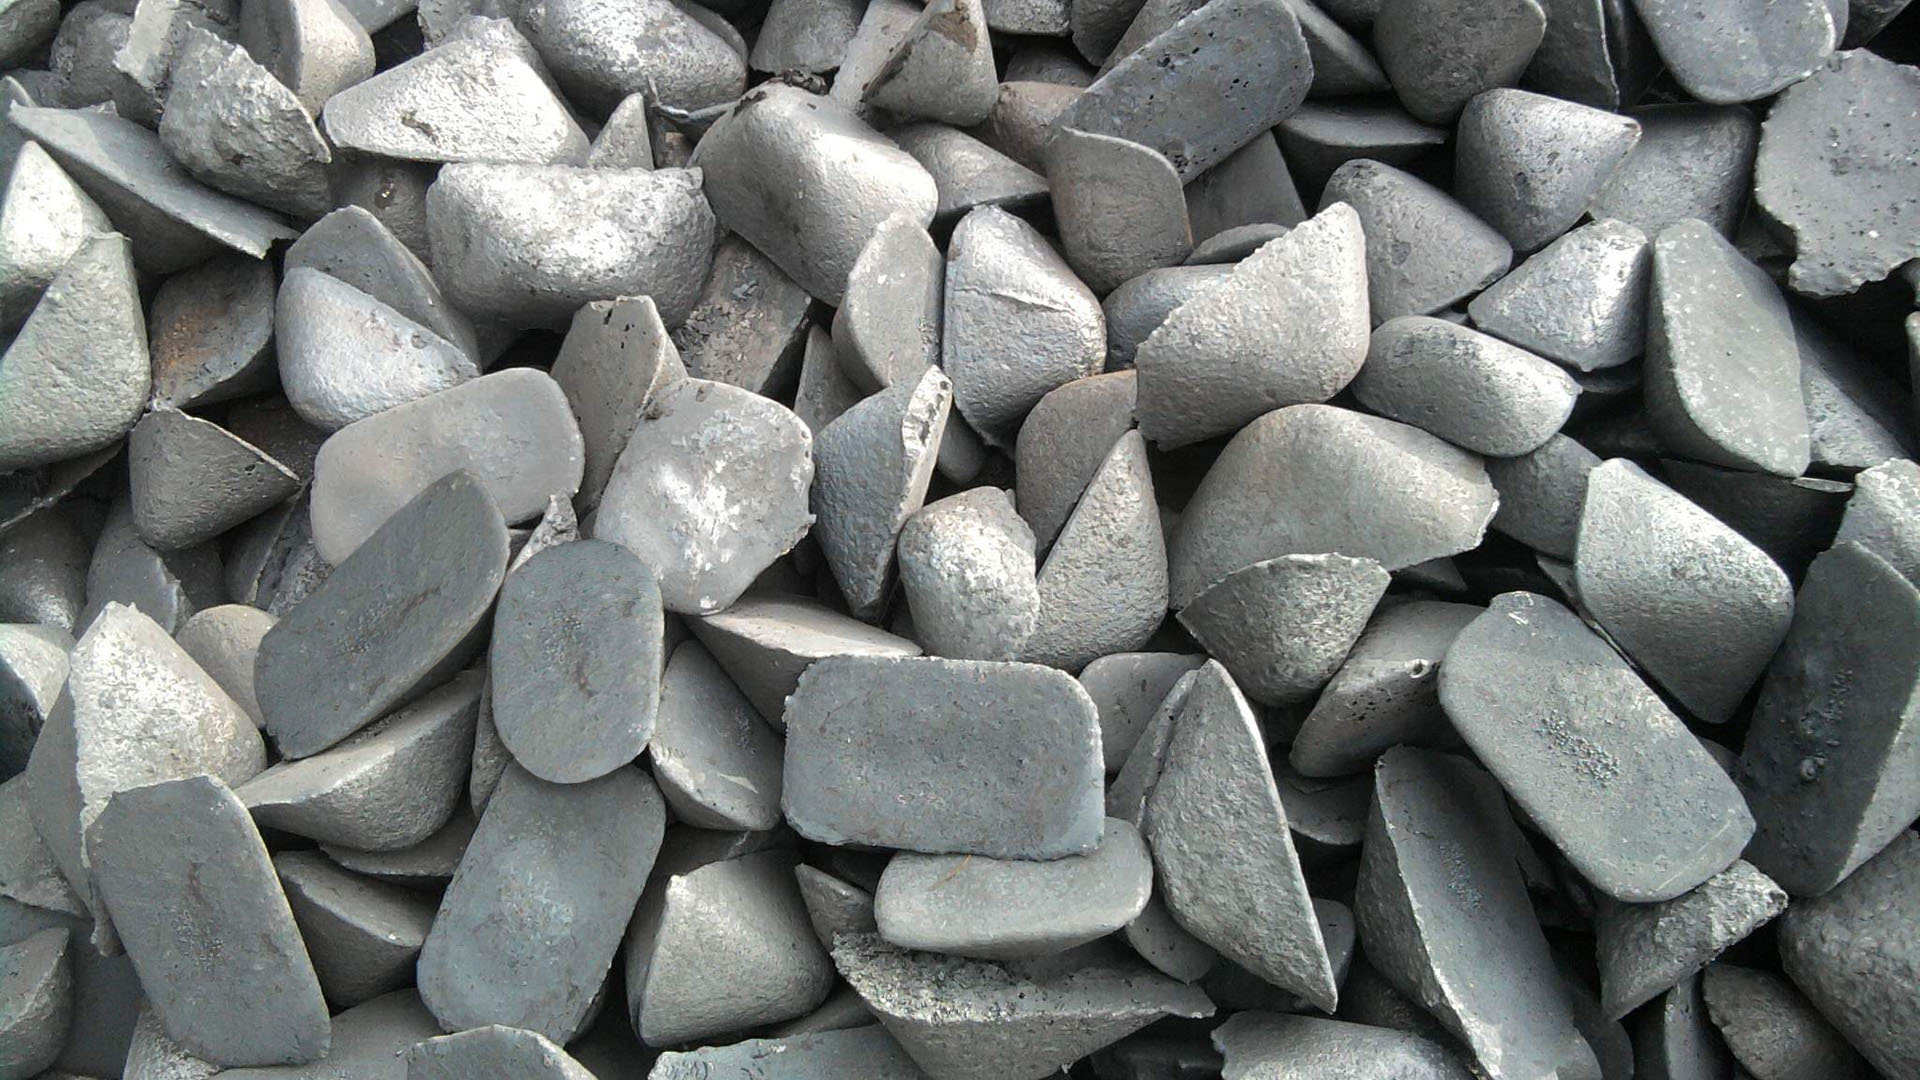
\includegraphics[width=0.7\textwidth]{Inagenes para latex/1 Arrabio.jpg}
    \caption{Arrabio encontrado en la naturaleza}
\end{figure}

\begin{itemize}
    \item \textbf{Características y propiedades:}
\end{itemize}

El arrabio se presenta en estado líquido a la salida del alto horno, con temperaturas $\approx \SI{1250}{\celsius} - \SI{1450}{\celsius}$. Debido a su elevado contenido de carbono y a la presencia de impurezas, es un material duro pero muy frágil, con baja tenacidad y escasa resistencia a los esfuerzos de tracción. Existen dos tipos principales: el arrabio gris, en el cual el carbono precipita en forma de grafito, lo que le otorga una apariencia grisácea y algo más de facilidad de mecanizado; y el arrabio blanco, donde el carbono está combinado químicamente en forma de cementita $Fe_3C$, lo que lo vuelve más duro y quebradizo.

\begin{itemize}
    \item \textbf{Usos:}
\end{itemize}

El arrabio no se utiliza de manera directa en aplicaciones industriales, sino que constituye la base para la producción de fundición o de acero. El arrabio gris suele destinarse a la fabricación de fundiciones grises en hornos de cubilote (En la sección \hyperref[cubilote_seccion]{3.2} se explicará más a detalle), mientras que el arrabio blanco se emplea como materia prima para fundiciones blancas o maleables y en hornos de afino (convertidores y hornos de oxígeno) para la obtención de acero.

\subsection{Fundición.}

\begin{itemize}
    \item \textbf{¿Qué es?}
\end{itemize}

 La fundición es una aleación de hierro y carbono cuyo contenido de carbono se sitúa entre 2,1\% y 4,5\%. Se obtiene a partir de la refundición del arrabio, generalmente en hornos como el cubilote, el crisol o el arco eléctrico. A diferencia del acero, la fundición conserva un mayor porcentaje de carbono, lo que modifica sus propiedades y determina que sea un material excelente para ser colado en moldes, de ahí su nombre.

\begin{figure}[H]
    \centering
    \begin{minipage}{0.47\textwidth}
        \centering
        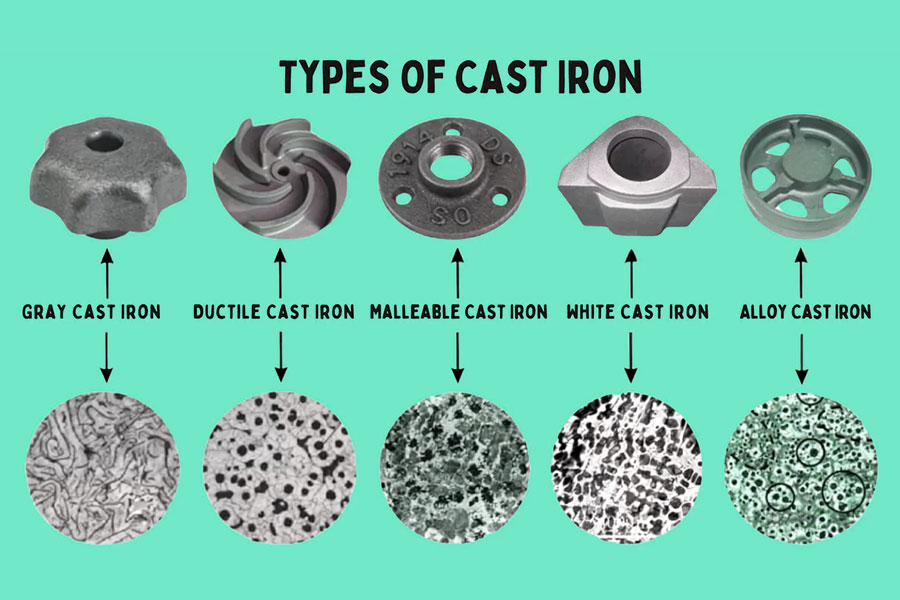
\includegraphics[width=\textwidth]{Inagenes para latex/Fundicion.png}
    \end{minipage}
    \begin{minipage}{0.47\textwidth}
        \centering
        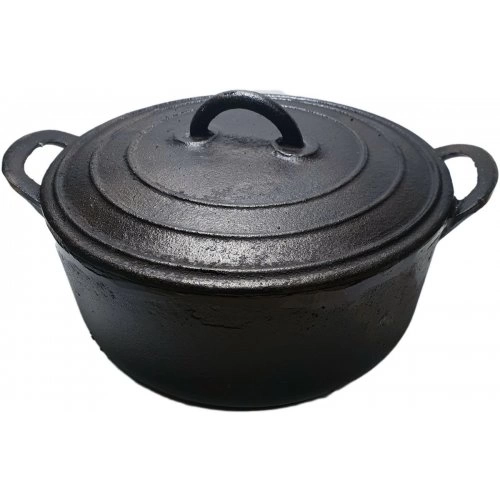
\includegraphics[width=\textwidth]{Inagenes para latex/fundicion 4.png}
    \end{minipage}
\end{figure}
 
\begin{itemize}
    \item \textbf{Características y propiedades:}
\end{itemize}

La fundición se caracteriza por su buena colabilidad, lo que permite obtener piezas complejas con gran detalle y acabado superficial. Posee una densidad ligeramente inferior a la del acero, una buena resistencia al desgaste y excelente amortiguación de vibraciones. Sin embargo, su alta cantidad de carbono le otorga fragilidad y la hace poco dúctil en comparación con el acero.
Existen varios tipos:

\begin{itemize}
    \item \textbf{Fundición gris:} con grafito laminar, de gran capacidad de mecanizado, muy usada en piezas de máquinas.
    \item \textbf{Fundición blanca:} con carbono en forma de cementita, muy dura y resistente al desgaste, pero frágil.
    \item \textbf{Fundición maleable:} obtenida a partir de la blanca mediante un recocido prolongado, lo que mejora su tenacidad
    \item\textbf{Fundición nodular o esferoidal:} con grafito en forma esférica, de gran resistencia y ductilidad.
    \item \textbf{Usos:}
\end{itemize}

La fundición gris se utiliza en bloques de motor, bancadas de máquinas, cañerías y tapas de alcantarilla. La fundición blanca se aplica en rodillos, molinos y piezas expuestas a abrasión. La maleable se usa en piezas de automóviles y accesorios de tuberías. La nodular, por su combinación de resistencia y ductilidad, se emplea en engranajes, cigüeñales, válvulas y piezas de maquinaria pesada.

\subsection{Acero.}
\begin{itemize}
    \item \textbf{¿Qué es?}
\end{itemize}

El acero es una aleación de hierro y carbono con un contenido de carbono comprendido entre 0,03\% y 2\%. Se obtiene a partir del arrabio mediante procesos de afino en convertidores (Bessemer, Thomas), hornos de reverbero (Siemens-Martin), hornos de oxígeno básico (LD, el más actual) o hornos de arco eléctrico (todos estos hornos se pueden apreciar en la \autoref{fig:hornos} y \autoref{fig:otros_hornos}). El objetivo del afino es eliminar el exceso de carbono y otras impurezas (como Si, Mn, N, etc.) para lograr un material con propiedades mecánicas equilibradas.

\begin{figure}[H]    
    \centering         
    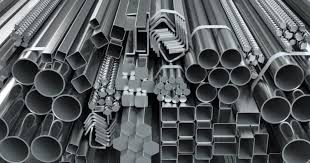
\includegraphics[width=0.6\textwidth]{Inagenes para latex/Acero.jpeg}
\end{figure}
\begin{itemize}
    \item \textbf{Características y propiedades:} 
\end{itemize}

El acero se distingue por su \textbf{ductilidad, tenacidad y maleabilidad}, propiedades que lo diferencian claramente de la fundición. Es más resistente a la tracción que la fundición y mucho menos frágil, lo que permite deformarlo en frío y en caliente para fabricar láminas, barras, perfiles y alambres. Sus propiedades varían enormemente según su composición: un acero dulce (con poco carbono, 0,1-0,2\%) es dúctil y fácil de trabajar, mientras que un acero de alta dureza (con carbono cercano al 1\%) es más resistente al desgaste pero menos maleable. Además, puede ser aleado con otros elementos (cromo, níquel, molibdeno, vanadio, entre otros) para obtener aceros inoxidables, resistentes al calor o de herramientas.

\begin{itemize}
    \item \textbf{Usos:}
\end{itemize}

El acero es el material estructural más utilizado en la industria moderna. Se emplea en la construcción de edificios, puentes y torres; en la industria automotriz para carrocerías, chasis y componentes mecánicos; en la fabricación de maquinaria, herramientas y electrodomésticos; y en la producción de tuberías, recipientes a presión y aceros especiales para aplicaciones químicas, médicas y nucleares.

\subsection{Mena.}
\begin{itemize}
    \item \textbf{¿Qué es?}
\end{itemize}

La mena es aquel mineral que contiene suficiente cantidad de hierro para que su extracción y procesamiento resulten económicamente rentables. Por ejemplo, la magnetita $(Fe_3O_4)$ y la hematita $(Fe_2O_3)$ son menas muy ricas, con porcentajes de hierro de aproximadamente 72\% y 69\% respectivamente. También se encuentran otros minerales como la siderita $(FeCO_3)$, que aunque contiene menos hierro ($\approx$ 58\%), se aprecia por su bajo contenido en fósforo y azufre, lo que la hace útil en procesos de afino. En otros casos aparece la pirita $(FeS_2)$, pero esta se descarta como fuente de hierro debido a su elevado contenido en azufre.

\begin{figure}[h!]
    \centering
    \begin{subfigure}{0.45\textwidth}
        \centering
        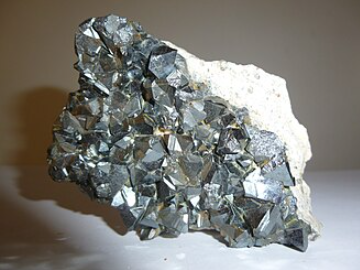
\includegraphics[width=\textwidth]{Inagenes para latex/magnetita.png}
        \subcaption{Magnetita}
        \label{magnetita}

        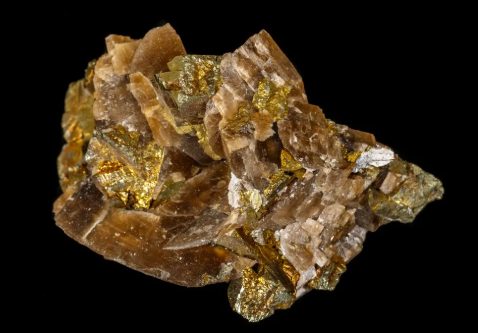
\includegraphics[width=\textwidth]{Inagenes para latex/siderita.png}
        \subcaption{Siderita}
        \label{siderita}
    \end{subfigure}
    \hfill
    \begin{subfigure}{0.45\textwidth}
        \centering
        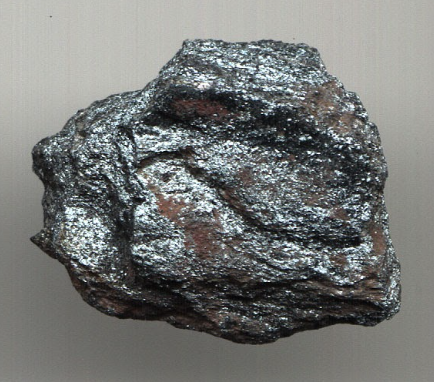
\includegraphics[width=\textwidth]{Inagenes para latex/hematita.png}
        \subcaption{Hematita}
        \label{hematita}

        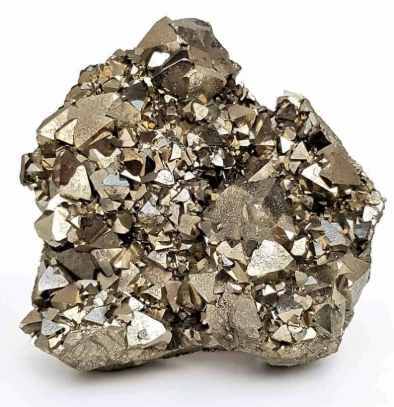
\includegraphics[width=\textwidth]{Inagenes para latex/pirita.png}
        \subcaption{Pirita}
        \label{pirita}
    \end{subfigure}
\end{figure}

\subsection{Ganga.}

\begin{itemize}
    \item \textbf{¿Qué es?}
\end{itemize}

La ganga hace referencia a la fracción de minerales y rocas sin valor metálico, que acompañan a la mena y deben ser eliminados mediante procesos de concentración. La ganga puede estar compuesta por sílice, arcillas, cuarzo u otros minerales.

\subsection{Piedra Caliza.}

\begin{itemize}
    \item \textbf{¿Qué es?}
\end{itemize}

Es una roca compuesta por carbonato de calcio $(CaCO_3)$. La piedra caliza reacciona químicamente con las impurezas de hierro fundido como azufre y fósforo, elevándolas a la parte superior de la mezcla de acero fundido, lo que permite separar correrctamente estas impurezas; así purifican el mineral de hierro y mejoran la calidad del producto final.

\subsection{Coque.}
\begin{itemize}
    \item \textbf{¿Qué es?}
\end{itemize}

Una planta de coque produce coque metalúrgico desde una mezcla de carbones. Se produce calentando el carbón a \SI{1250}{\celsius} en una atmósfera libre de oxígeno. El coque producido se compone de más de un 90\% de C, que se emplea como suministro energético y agente químico en el alto horno.

\section{Obtención del Arrabio.}

Una vez que la mena es seleccionada y mediante un proceso es preparada, se da inicio al proceso de reducción para obtener el primer producto metálico: el arrabio. Este se fabrica en el alto horno, cuyo funcionamiento es continuo, lo que significa que puede operar durante años sin interrupciones, recibiendo constantemente mineral de hierro, coque y caliza por la parte superior. El coque actúa simultáneamente como combustible y reductor químico, ya que al reaccionar con el aire caliente inyectado por las toberas en la base del horno genera CO (esto se aprecia en la \autoref{fig:alto_horno}). Este gas asciende por la columna de carga y reduce progresivamente los óxidos de hierro presentes en el mineral. Mientras tanto, el fundente (caliza) se descompone en óxido de calcio, que se combina con impurezas como la sílice para formar escoria. De este modo, en la parte baja del horno se acumula una capa de hierro fundido, llamada arrabio, cubierta por la escoria flotante que lo protege de la oxidación. Periódicamente, tanto el hierro como la escoria se extraen a través de orificios llamados piqueras. 

El arrabio resultante contiene entre 3 y 4,5\% de carbono, además de fósforo, azufre, manganeso y silicio, lo que lo convierte en un material frágil y de uso limitado en su forma directa.

Posteriormente, el arrabio se puede transformar en fundición gris en hornos de cubilote, donde parte del carbono se precipita en forma de grafito.
El arrabio blanco, en cambio, contiene carbono principalmente disuelto en forma de cementita, lo que lo hace frágil y duro. Puede ser transformado en fundición blanca o maleable mediante hornos de refinación o de arco eléctrico.

Por ende, la obtención del arrabio en alto horno es el método tradicional y principal, donde el mineral se funde y se reduce con $CO$ generado por la combustión del coque, siendo el producto resultante el arrabio líquido.
Este proceso se llama reducción indirecta porque el oxígeno del mineral se elimina principalmente gracias al monóxido de carbono como agente reductor intermedio, no directamente con el carbono sólido.

También existen otros métodos modernos que se llaman de reducción directa (DRI\footnote{Direct Reduced Iron, en español: hierro reducido directamente}), aquí no se usa alto horno ni coque, sino gas natural reformado $(CO + H_2)$ o carbón pulverizado, donde el mineral se reduce en estado sólido, sin llegar a fundirse. En este caso el producto no es arrabio líquido, sino hierro esponja (o DRI), que luego se funde en hornos de arco eléctrico para hacer acero. Este proceso sí se llama reducción directa, porque el oxígeno se elimina directamente con $CO + H_2$ sin pasar por una etapa de fusión.

Otros procesos alternativos como: Corex, Finex, Hismelt. Estos producen arrabio líquido como el alto horno, pero sin usar coque, aprovechando carbón mineral y gases reductores. No son reducción directa pura, pero tampoco son el alto horno clásico: se consideran tecnologías intermedias o alternativas.

\begin{figure}[H]    
    \centering         
    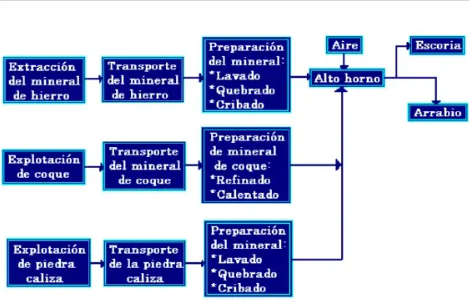
\includegraphics[width=0.9\textwidth]{Inagenes para latex/obtencion de arrabio.png}
\end{figure}

\subsection{Método Conceptual.}

\begin{itemize}
    \item \textbf{Carga:} mineral de hierro (2 t), coque (1 t), caliza (0.5 t) y aire (4 t).
    \item \textbf{Producto:} arrabio (1 t, con composición típica: Fe 93,7\%; C 4,5\%; Mn 0,4\%; Si 0,45\%; P 0,11\%; S 0,025\%), escoria (0.5 t) y gases (6 t).
    \item \textbf{Temperaturas:} desde 200°C en la parte superior hasta 1500°C en la zona de fusión.
    \item \textbf{Eficiencia:} se mejora con aire precalentado (1030°C) y enriquecido en oxígeno, reduciendo pérdidas térmicas.
\end{itemize}

\subsection{Horno Asociado.} \label{alto_horno}

\textbf{Tipo: Alto Horno (Blast Furnace).}

\begin{itemize}
    \item \textbf{Uso:} reducción de minerales de hierro en estado sólido para producir arrabio líquido. Es un horno continuo de gran capacidad (hasta 5000 t/día), con estructura cilíndrica refractaria, toberas para inyección de aire caliente y regeneradores para precalentar el aire.
    \item \textbf{Características:} es una estructura monumental de forma cilíndrica, con una altura de entre 20 y 40 metros, revestida con ladrillos refractarios capaces de soportar temperaturas superiores a \SI{1600}{\celsius}, funciona a contracorriente (carga por arriba, gases por debajo). Asociado a procesos como sinterización de minerales y producción de coque. Su funcionamiento es continuo, lo que significa que puede operar durante años sin interrupciones, recibiendo constantemente mineral de hierro, coque y caliza.
\end{itemize}

\begin{figure}[h!]
    \centering
    \begin{subfigure}{0.45\textwidth}
        \centering
        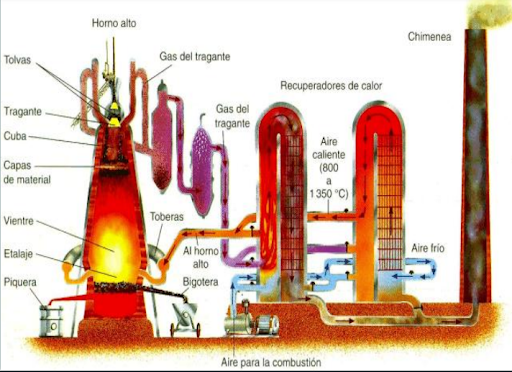
\includegraphics[width=\textwidth]{Inagenes para latex/Alto horno.png}
    \end{subfigure}
    \hfill
    \begin{subfigure}{0.45\textwidth}
        \centering
        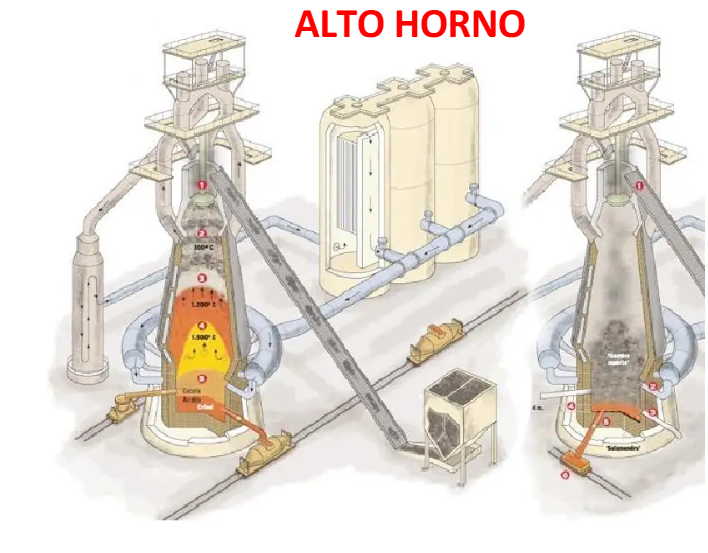
\includegraphics[width=\textwidth]{Inagenes para latex/alto horno 2.png}
    \end{subfigure}
    \caption{Esquema de un Alto Horno.}
    \label{fig:alto_horno}
\end{figure}

\section{Obtención de Fundición.}

La fundición se obtiene a partir de la refusión del arrabio en hornos específicos, a los cuales se le puede añadir chatarra metálica y fundentes según las propiedades buscadas en el producto final. El proceso comienza con la carga del arrabio sólido (en lingotes) o líquido proveniente del alto horno, junto con coque como combustible y piedra caliza como fundente (en el caso del cubilote). La función del coque es doble: aportar calor por combustión e introducir $CO$, que actúa como reductor secundario. En los hornos de arco eléctrico o crisol, la energía de fusión proviene de la electricidad o del calor transmitido indirectamente, lo que brinda un mayor control químico.

Durante la fusión, la temperatura se eleva entre \SI{1350}{\celsius} y \SI{1500}{\celsius}, lo suficiente para mantener el hierro en estado líquido y permitir la formación de escoria. A diferencia del acero, en el proceso de obtención de fundición no se busca reducir el carbono, sino mantener un contenido elevado (2,1-4,5\%). De hecho, en muchos casos se añade carbono extra (por ejemplo, en forma de coque o aditivos carbonosos) para ajustar la composición. Asimismo, es frecuente introducir elementos de aleación (silicio, manganeso, níquel, cromo, magnesio) que modifican la microestructura y dan lugar a fundiciones con propiedades específicas.

El comportamiento del carbono durante el enfriamiento determina el tipo de fundición obtenida:

\begin{itemize}
    \item Si el enfriamiento es relativamente lento, el carbono precipita en forma de grafito, dando lugar a la fundición gris (grafito laminar).
    \item Si el enfriamiento es rápido, el carbono queda combinado en forma de cementita $(Fe_3C)$, originando la fundición blanca.
    \item Si la fundición blanca se somete a un recocido prolongado (varios días a temperaturas entre 900-950 °C), el carbono combinado se descompone y parte de él precipita como grafito irregular, transformándola en fundición maleable.
    \item Si durante la fusión se añade magnesio o cerio, el grafito se nuclea en forma de esferas, lo que genera la fundición nodular o esferoidal, con una microestructura mucho más tenaz y resistente.
\end{itemize}

Por lo tanto, la obtención de fundición implica no solo la simple fusión del arrabio, sino también el control del horno, de la atmósfera de fusión, de los aditivos y de la velocidad de enfriamiento, lo que permite orientar la microestructura hacia grafito laminar, cementita, grafito esferoidal o combinaciones intermedias. Este control microestructural es lo que explica la gran variedad de fundiciones y su amplio rango de aplicaciones industriales.

\subsection{Método Conceptual.}
\begin{itemize}
    \item \textbf{Carga:} arrabio, chatarra, coque y fundentes.
    \item \textbf{Reacciones:} fusión y ajuste de $ C/Si$ para formar grafito o cementita. Reducción de $S/P$.
    \item \textbf{Producto:} fundición gris (maleable, usada en piezas fundidas) o blanca (dura, para laminación).
\end{itemize}

\subsection{Hornos Asociados} \label{cubilote_seccion}

\textbf{Tipo: Horno de cubilote.}

\begin{itemize}
    \item \textbf{Uso:} es el más utilizado en fundiciones tradicionales por su bajo costo operativo.
    \item \textbf{Características:} tiene forma cilíndrica y funciona con coque como combustible, aire comprimido y cargas de arrabio y chatarra. Puede considerarse un alto horno en miniatura, capaz de mantener una producción continua de fundición gris.
\end{itemize}

\textbf{Tipo: Horno de Crisol.}

\begin{itemize}
    \item \textbf{Uso:} se emplea para producciones más reducidas y para aleaciones especiales. En él, el metal se coloca dentro de un recipiente refractario que se calienta externamente mediante carbón, gas o electricidad. Por su versatilidad y control de impurezas, es ideal para lotes pequeños o pequeñas fundiciones.
    \item \textbf{Características:} esta constituido de un crisol hecho de material refractario, como grafito, hecho para contener el material que se va a fundir y el cual soporta temperaturas extremadamente altas. El crisol se calienta mediante aplicación de calor desde el exterior, que puede ser mediante combustibles sólidos como coque, gaseosos como gas natural, propano, electricidad u otros medios.
\end{itemize}

\textbf{Tipo: Horno de Arco Eléctrico.}

\begin{itemize}
    \item \textbf{Uso:} se utiliza tanto en fundiciones especiales como en la producción de aceros aleados e inoxidables.
    \item \textbf{Características:} su principio de funcionamiento se basa en la generación de un arco eléctrico entre uno o varios electrodos de grafito y la carga metálica. Este arco produce temperaturas extremadamente altas ($+ \SI{3000}{\celsius}$ en la zona del arco), suficientes para fundir chatarra, arrabio sólido, hierro esponja (DRI) o una combinación de ellos.
\end{itemize}

\begin{figure}[h!]
    \centering
    \begin{subfigure}{0.9\textwidth}
        \centering
        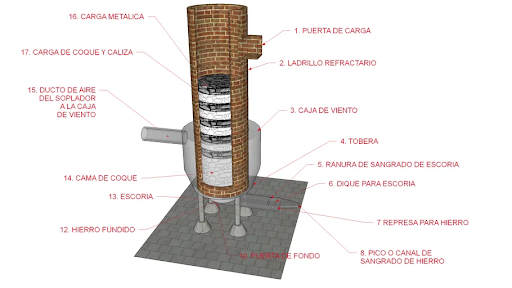
\includegraphics[width=\textwidth]{Inagenes para latex/cubilote.png}
        \subcaption{Horno de Cubilote}
        \label{cubilote}
    \end{subfigure}
    \begin{subfigure}{0.45\textwidth}
        \centering
        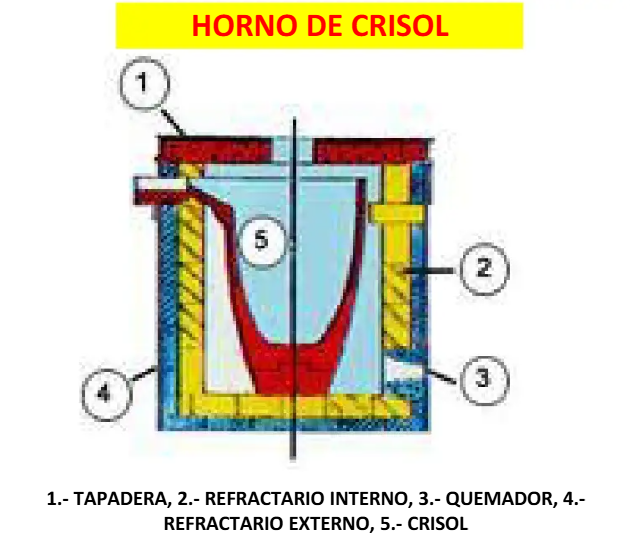
\includegraphics[width=\textwidth]{Inagenes para latex/crisol.png}
        \subcaption{Horno de Crisol}
        \label{crisol}
    \end{subfigure}
    \hfill
    \begin{subfigure}{0.45\textwidth}
        \centering
        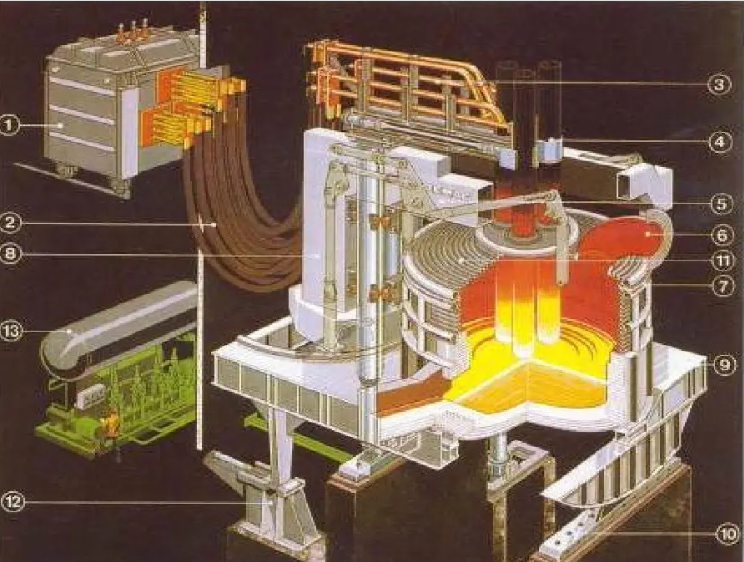
\includegraphics[width=\textwidth]{Inagenes para latex/arco electrico.png}
        \subcaption{Horno de Arco Eléctrico}
        \label{electrico}
    \end{subfigure}
    \caption{Tipos de hornos.}
    \label{fig:hornos}
\end{figure}

\section{Obtención del Acero.}

En general el conjunto de procesos para convertir el arrabio en acero se denomina afino. El afino se puede realizar en distintos aparatos. Entre los tipos de aparatos que se emplean están los llamados convertidores.
Un convertidor es un gran recipiente en forma de pera, revestido interiormente de material refractario, cuyo fondo está perforado. Mientras se vierte la colada líquida, el convertidor se mantiene en posición horizontal para evitar que el líquido alcance los orificios del fondo. Una vez que se ha completado la carga, el convertidor se endereza, al mismo tiempo que comienza el soplado de aire a 2-3 atm de presión a través de los orificios del fondo. El oxígeno del aire oxida al hierro formando $FeO$. Este se disuelve y oxida al silicio y al manganeso. Los óxidos formados reaccionan con el $SiO_2$ y con el revestimiento formando una escoria que flota sobre el material fundido. Luego, comienza la oxidación del carbono. Cuando el $CO$ llega a la atmósfera se observan llamaradas de 7 a 9 metros en la boca del convertidor, alcanzando en el interior una temperatura de \SI{1600}{\celsius}. Una rápida disminución en el largo de la llama revela que la descarburación ha terminado. El proceso en el convertidor dura unos 20 minutos durante los que se pueden afinar de 10 a 25 toneladas de arrabio. Esta rapidez no permite un control muy exacto del proceso y, por lo tanto, de la composición final del acero.

\begin{figure}[h!]    
    \centering         
    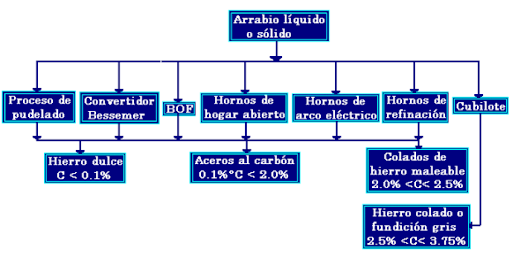
\includegraphics[width=1\textwidth]{Inagenes para latex/Diagrama de acero.png}
\end{figure}

\subsection{Método Conceptual.}

\begin{itemize}
    \item \textbf{Carga típica:} arrabio (93\% Fe; 4\% C; 0,5-2\% Si; 1\% Mn; 2-0,1\% P; 0,05\% S) + chatarra + fundentes.
    \item \textbf{Metalurgia secundaria:} agitación (con argón o EMS), desgasificación (RH o tanque), horno cuchara para recalentamiento y ajustes.
    \item \textbf{Producto:} acero con Fe 98\%; C 0,05-1,5\%; Si 0,5-2\%; Mn 0,3-0,6\%; P/S < 0,05\%.
\end{itemize}

\subsection{Hornos Asociados.}

\textbf{Tipo:  Convertidores Bessemer.}

\begin{itemize}
    \item \textbf{Características:} 
    El proceso es similar al del LD, con la diferencia de que se introduce una mezcla de oxígeno y nitrógeno (aire); el nitrógeno produce nitruros de hierro que, a pesar de estar presentes en pequeñas cantidades, proporcionan dureza y fragilidad al acero. Es un método antiguo que prácticamente ya no se utiliza. El convertidor Bessemer o de pared ácida, que se usa cuando no existen impurezas de azufre o fósforo.
\end{itemize}

\textbf{Tipo: Convertidores Thomas.}

\begin{itemize}
    \item \textbf{Características:} es una modificación del convertidor Bessemer. Se caracteriza porque la cubata está revestida con una mezcla  de materiales de PH básicode dolomía y alquitrán, que permitía eliminar del acero el fósforo presente en el mineral de hierro. El fósforo contenido en el arrabio, se conbinaba con la caliza presente en el  mineral de hierro.
\end{itemize}

\textbf{Tipo: Hornos de Oxígeno (LD).}

\begin{itemize}
    \item \textbf{Características:} 
    Sobre el arrabio fundido se hace incidir un chorro de oxígeno puro insuflado en sentido vertical y a presión. Es un proceso muy rápido que requiere un control automatizado de las cargas de arrabio y de fundente que se utilizan y de la presión y el caudal del oxígeno. Al insuflar oxígeno sobre el arrabio se genera óxido ferroso $(FeO)$,el cual reacciona con las impurezas y forma óxidos, con los que se eliminan estas impurezas. Luego, se añade rápidamente fundente y se sigue insuflando oxígeno que forma monóxido de carbono $(CO)$ y dióxido de carbono $(CO_2)$, y de manera que se reduce el contenido de carbono, hasta llegar al grado de composición deseado.
    Este procedimiento es uno de los más modernos y el más utilizado en la actualidad porque permite obtener aceros de muy buena calidad, es relativamente sencillo y de bajo costo.
\end{itemize}

\textbf{Tipo: Hornos Siemens-Martin.}

\begin{itemize}
    \item \textbf{Características:} 
    Son hornos de reverbero revestidos interiormente de material refractario ácido o básico, según la naturaleza del material de afino. Utilizan como combustible aceite combustible o gas de coque. El ciclo de fabricación del acero se inicia dejando mineral de hierro y fundente y/o chatarra en los hornos. Al comenzar la fusión, se agrega arrabio líquido o en lingotes. Cuando funde toda la carga se realizan sucesivos controles químicos y de temperatura, a fin de efectuar los ajustes necesarios que den al acero las especificaciones previstas. Al cabo de varias horas se destapa el orificio de colada y el acero fluye a través de un canal, llenando un recipiente llamado cuchara de colada. Eventualmente, a este recipiente se le agregan materiales de aleación para obtener aceros especiales. En la cuchara de colada la escoria excedente sobrenada el acero, se la elimina dejándola fluir a través de un canal de desborde hacia un recipiente llamado pote de escoria. 
    Desde la cuchara de colada y a través de un orificio ubicado en su fondo, llamado buza, el acero es vaciado en lingoteras de formas y tamaños apropiados.
\end{itemize}

\textbf{Tipo: Hornos de Inducción.}

\begin{itemize}
    \item \textbf{Características:} 
    un horno eléctrico que funciona gracias al principio de la inducción electromagnética. En lugar de calentar el metal con un arco eléctrico o con la combustión de un combustible, el horno utiliza corrientes inducidas dentro del propio metal para fundirlo.
    El equipo está formado por un crisol refractario rodeado por una bobina de cobre refrigerada por agua. Al hacer pasar una corriente alterna de alta frecuencia por la bobina, se genera un campo electromagnético variable que induce corrientes parásitas (corrientes de Foucault) en la carga metálica. Estas corrientes circulan dentro del metal y lo calientan hasta fundirlo.
\end{itemize}

 \begin{figure}[h!]
    \centering
    \begin{subfigure}{0.45\textwidth}
        \centering
        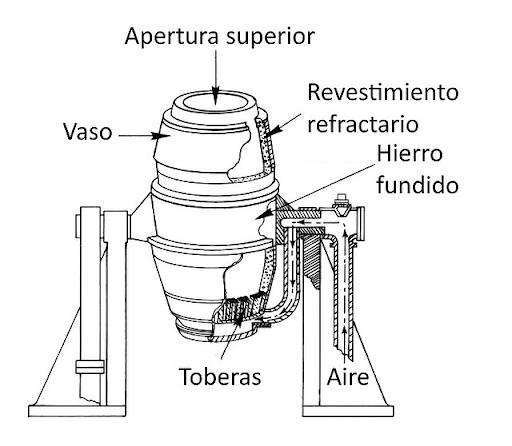
\includegraphics[width=\textwidth]{Inagenes para latex/convertidor baser.png}
        \subcaption{Horno Bessemer}
        \label{bessemer}

        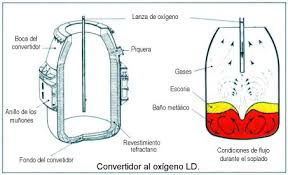
\includegraphics[width=\textwidth]{Inagenes para latex/bof1.png}
        \subcaption{Horno de oxígeno (LD)}
        \label{LD}
    \end{subfigure}
    \hfill
    \begin{subfigure}{0.45\textwidth}
        \centering
        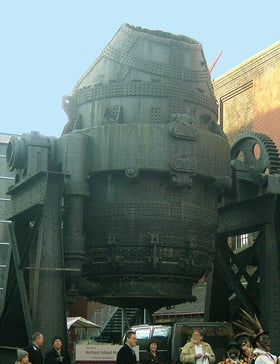
\includegraphics[width=\textwidth]{Inagenes para latex/convertidor tamas.png}
        \subcaption{Horno Thomas}
        \label{thomas}

        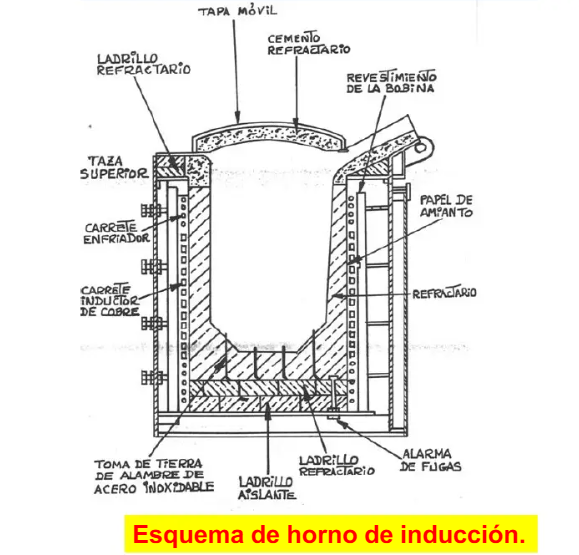
\includegraphics[width=\textwidth]{Inagenes para latex/induccion 2.png}
        \subcaption{Horno de Inducción}
        \label{induccion}
    \end{subfigure}
    \caption{Otros tipos de hornos.}
    \label{fig:otros_hornos}
 \end{figure}

\section{Conclusión}
La comparación de estos hornos y procesos muestra cómo la siderurgia evolucionó desde sistemas rudimentarios hasta complejos altamente eficientes. El alto horno es esencial para obtener arrabio a gran escala; los hornos de cubilote, crisol y arco eléctrico diversifican la producción de fundiciones; y los convertidores Bessemer, Thomas, Siemens-Martin, LD y hornos de arco eléctrico marcan la historia y la actualidad de la producción de acero. Cada horno tiene un papel particular dentro de la cadena de producción: el alto horno para la reducción de minerales, el cubilote para fundiciones económicas, el crisol para aleaciones especiales, el arco eléctrico para fundiciones y aceros de alta precisión, y los convertidores para el afino masivo del arrabio en acero.

La obtención de arrabio, fundición y acero constituye una cadena productiva compleja que comienza con la extracción de la mena y su separación de la ganga, continúa con la reducción en el alto horno y se diversifica en fundiciones o aceros según el tipo de horno utilizado. El conocimiento detallado de los hornos industriales es esencial, ya que cada uno aporta ventajas y limitaciones específicas. Mientras que el alto horno es el corazón de la producción primaria, hornos como el cubilote o el LD representan la especialización y modernización de la industria siderúrgica.

\vfill
\textit{\textbf{Este trabajo fue elaborado con la ayuda de la IA y otras páginas de ayuda para facilitar la confección y disposición de los elementos en dicho trabajo; y la búsqueda de información para complementar la dada por la cátedra.}}

\newpage
\section{Bibliografía}
\begin{itemize}
    \item \url{https://es.wikipedia.org/wiki/Mena_(miner%C3%ADa)}
    \item \url{https://es.wikipedia.org/wiki/Ganga_(miner%C3%ADa)}
    \item \url{https://es.wikipedia.org/wiki/Magnetita}
    \item \url{https://es.wikipedia.org/wiki/Magnetita}
    \item \url{https://geologiaweb.com/minerales/hematita/}
    \item \url{https://es.wikipedia.org/wiki/Siderita}
    \item \url{https://emersonrincon.blogspot.com/2015/10/hornos.html}
    \item \url{http://recursosbiblio.url.edu.gt/Libros/2013/cmII/3.pdf}
    \item \url{http://www.eet485.com.ar/Archivos/Conocimiento%20de%20los%20materiales%203eros_z5j.pdf}
    \item \url{https://www.youtube.com/watch?v=s1Lr0fpTj-0}
    \item \url{lhttps://metalurgia.usach.cl/sites/metalurgia/files/documentos/capitulo08fab-aceros.pdf}
    \item Aguilar Schafer, J.A. Yacimientos minerales y procesos geológicos.
    \item Aguilar Schafer, J.A. Explotación minera, preparación y concentración.
    \item Aguilar Schafer, J.A. Metalurgia extractiva del hierro.
    \item Aguilar Schafer, J.A. Hornos Industriales.
\end{itemize}

\end{document}